\documentclass[12pt,a4paper,twopage]{article}
\usepackage[utf8]{inputenc}
\usepackage[a4paper,margin=1cm,footskip=.5cm]{geometry}
\usepackage{multicol}
\usepackage{amsmath}
\usepackage{float}
\usepackage{epsfig,graphicx}
\usepackage{xcolor,import}
\usepackage{subcaption}
\usepackage[font=small,labelfont=bf]{caption}
\usepackage{siunitx}
\usepackage[german]{babel}
\usepackage{textcomp}
\usepackage{mathtools}
\linespread{1.1}
\usepackage{parskip}
\setlength{\parindent}{12pt}

\begin{document}


\thispagestyle{empty}
			\begin{center}
			\Large{Fakultät für Physik}\\
			\end{center}
\begin{verbatim}


\end{verbatim}
							%Eintrag des Wintersemesters
			\begin{center}
			\textbf{\LARGE SOMMERSEMESTER 2015}
			\end{center}
\begin{verbatim}


\end{verbatim}
			\begin{center}
			\textbf{\LARGE{Physikalisches Praktikum II}}
			\end{center}
\begin{verbatim}




\end{verbatim}

			\begin{center}
			\textbf{\LARGE{PROTOKOLL}}
			\end{center}
			
\begin{verbatim}





\end{verbatim}

			\begin{flushleft}
			\textbf{\Large{Experiment (Nr., Titel):}}\\
							%Experiment Nr. und Titel statt den Punkten eintragen
			\LARGE{11: Hall-Effekt}	
			\end{flushleft}

\begin{verbatim}

\end{verbatim}	
							%Eintragen des Abgabedatums, oder des Erstelldatums des Protokolls
			\begin{flushleft}
			\textbf{\Large{Datum:}} \Large{12.06.2015}
			\end{flushleft}
			
\begin{verbatim}
\end{verbatim}
							%Namen der Protokollschreiber
		\begin{flushleft}
			\textbf{\Large{Bachleitner Veronika, Grafendorfer Erik}} 
			\end{flushleft}

\begin{verbatim}


\end{verbatim}
							%Kurstag und Gruppennummer, zb. Fr/5
			\begin{flushleft}
			\textbf{\Large{Kurstag/Gruppe:}} \Large{FR/1}
			\end{flushleft}

\begin{verbatim}






\end{verbatim}
							%Name des Betreuers, das Praktikum betreute.
			\begin{flushleft}
			\LARGE{\textbf{Betreuer:\Large{ KLEPP }}}		
			\end{flushleft}
			
\pagebreak			
			
\section{Aufgabenstellung}
Wir untersuchen verschiedene Größen die beim Halleffekt in Halbleitern auftreten.
\section{Theorie}

Aus der Längsspannung am Halbleiter und dem Strom durch ihn ergibt sich der Widerstand R des Leiters.

Aus R ergeben sich mit der Länge l und der Fläche A des Leiters der spezifische Widerstand $\rho$ und die Leitfähigkeit $\sigma$:

$$ R = \rho \frac{l}{A} $$

$$ \sigma = \frac{1}{\rho} $$
$$ \sigma = n \cdot q \cdot \mu $$

Damit ergeben sich für $\sigma$ und $\mu$ :

$$ \sigma = \frac{1}{R} \frac{l}{A} $$

$$ \mu = \frac{\sigma}{n \cdot q} $$

n ergibt sich aus der Hallkonsante:

$$ n = -\frac{1}{q\cdot R_H} $$

Wobei q die Elementarladung bedeutet.


Der lineare Fit durch den Plot der Hallspannung gegen die variierte Probenstromstärke $I_{Probe}$ ergibt einen Fitparameter $\alpha$, aus dem wir einen ersten Wert für $R_H$ erhalten:

\begin{equation}
\label{afit}
\begin{split}
U_H(I_{Probe})& = \alpha I \\
U_H(I_{Probe})& = \frac{R_H B}{d} I \\
\rightarrow \alpha & = \frac{R_H B}{d} \\
\rightarrow R_H & = \frac{\alpha d}{B}
\end{split}
\end{equation}

Der lineare Fit durch den Plot der Hallspannung in Abhängigkeit der magnetischen Flussdichte liefert uns einen Parameter $\beta$, der sich wie folgt darstellt:

\begin{equation}\label{bfit}
\begin{split}
U_H(B)& = R_H \frac{I B}{d} \\
U_H(B)& = \beta B \\
\rightarrow \beta & = \frac{I R_H}{d} \\
\rightarrow R_H & = \frac{\beta d}{I}
\end{split}
\end{equation}



\section{Aufbau}

\section{Durchführung}
Aus der relativen Unsicherheit des Abstandes zwischen den Polschuhen ($\frac{\Delta d}{d}= \frac{0.2}{10} = 0.02 $ erhalten wir auch die relative Unsicherheit des B-Feldes:  0.02. Dazu kommt aber noch die Unsicherheit durch die Erzeugung des B-Feldes mit dem Netzgerät, die $\pm$ 1 mA beträgt - und die relative Unsicherheit der Relation zwischen der erzeugenden Stromstärke des B-Feldes, die $\frac{0.25}{48.7}$ beträgt. In den Plots und den Fits wurden alle berücksichtigt. 

Für die Unsicherheit der Hallspannung wurde nur die Digitalisierungsunsicherheit des Multimeters berücksichtigt. 

Für zusammengesetzte Unsicherheiten wurde die Gaußsche Fehlerfortpflanzung angewandt.
\section{Ergebnisse}
\subsection*{}

\begin{figure}
\begin{center}

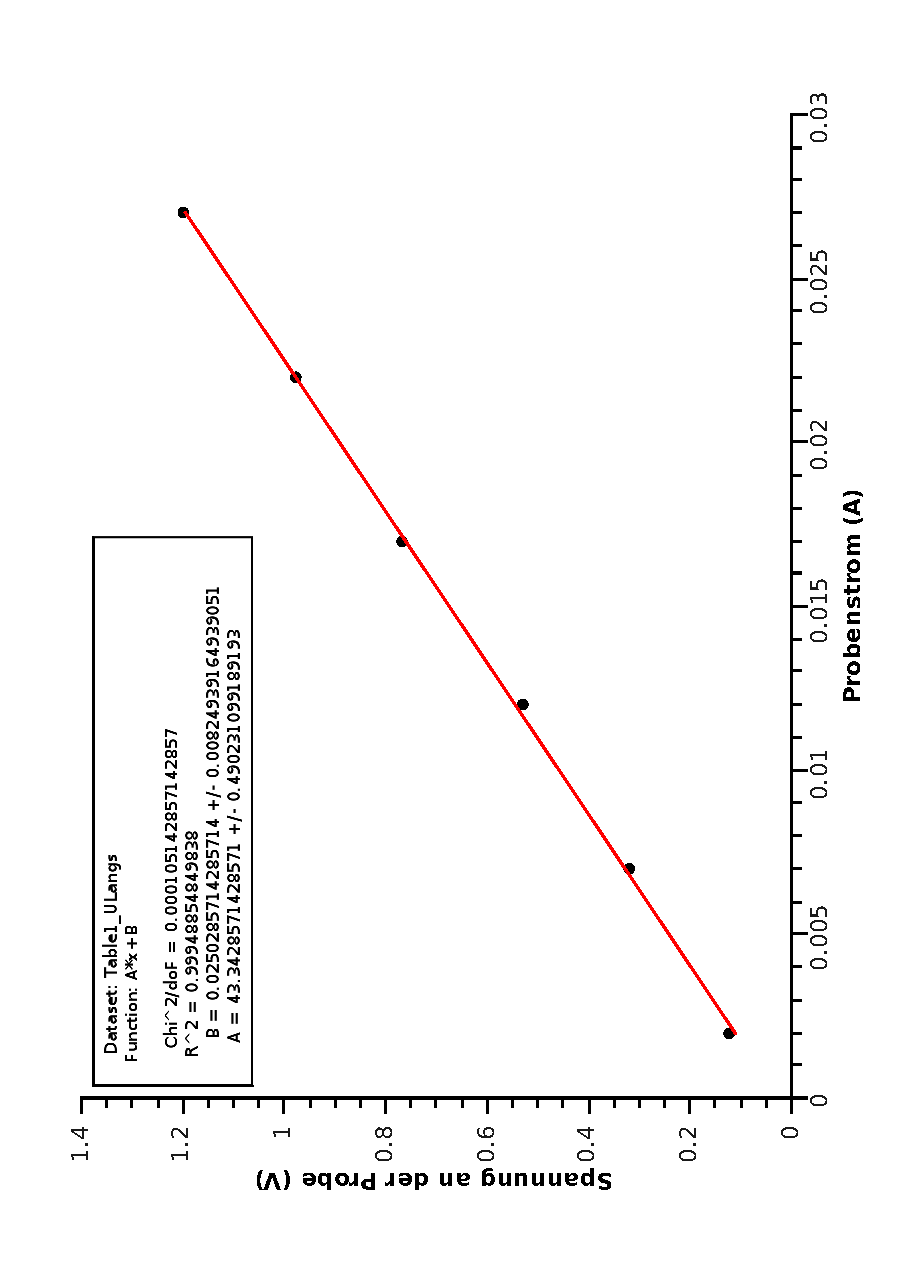
\includegraphics[width=0.4\linewidth, angle=-90]{widerstand.eps}
\caption{Widerstandsbestimmung durch linearen Fit}
\end{center}
\end{figure}

Aus dem linearen Fit durch die Längsspannung in Abhängigkeit des Probenstroms ergibt sich direkt der Widerstand des Halbleiters als Steigung der Gerade:

\begin{center}


$$R = (43.3 \pm 0.5) \Omega $$

$$\rho = (0.02165 \pm 0.00025) \Omega m^{-1} $$

$$\sigma =  46.2 \pm 0.6 $$  

\end{center}
\subsection*{Magnetowiderstand}
Table5: 0,70659142 +/- 0,017301197
$R_{Rel} = \frac{\Delta R(B)-R(B=0)}{R(B=0)}$
\begin{table}
\begin{tabular}{|c|c|c|c|c|}
\hline 
$I_B$ & $R_{Rel}$ \\
\hline  & $n-Ge \vec{B}$ & $n-Ge -\vec{B}$ & $p-Ge \vec{B}$ & $p-Ge -\vec{B}$ \\
0.5 & 0.0558 & 0.0586 & 0.3551 & 0.3515 \\ 
1 & 0.0558 & 0.0586 & 0.3561 & 0.3533 \\ 
1.5 & 0.0568 & 0.0595 & 0.3588 & 0.3561 \\ 
2 & 0.0577 & 0.0605 & 0.3625 & 0.3598 \\ 
2.5 & 0.0586 & 0.0614 & 0.3662 & 0.3644 \\ 
3 & 0.0605 & 0.0632 & 0.3718 & 0.3699 \\ 
3.5 & 0.0623 & 0.0642 & 0.3764 & 0.3755 \\ 
4 & 0.0642 & 0.0660 & 0.3819 & 0.3810 \\ 
4.5 & 0.0660 & 0.0678 & 0.3884 & 0.3866 \\ 

\end{tabular}
\end{table}


Laut (\ref{afit}) gibt qtiplot für $\alpha$:

$$ \alpha = 1.88 \pm 0.05 $$

Daraus mit (\ref{afit}) nach $R_H$:

\begin{center}
$$ \boxed{ R_H(I_{Probe}) = 0.0125 \pm 0.0006 } $$
\end{center}

Daraus ergibt sich für n:

\begin{center}
$$ \boxed{ n_{IProbe} = (5.0 \pm 0.3) \cdot 10^{20}  } $$
\end{center}

Laut (\ref{bfit}) gibt qtiplot für $\beta$:

$$ \beta =  0.206 \pm 0.006 $$

Daraus erhalten wir mit (\ref{bfit}) für $R_H$:

\begin{center}
$$ \boxed{ R_H(B) = 0.0082 \pm 0.0005 } $$
\end{center}

\begin{center}
$$ \boxed{ n_{B} = (7.6 \pm 0.5) \cdot 10^{20}  } $$
\end{center}

$$ \sigma = $$



\pagebreak

\begin{figure}[H]
\begin{center}
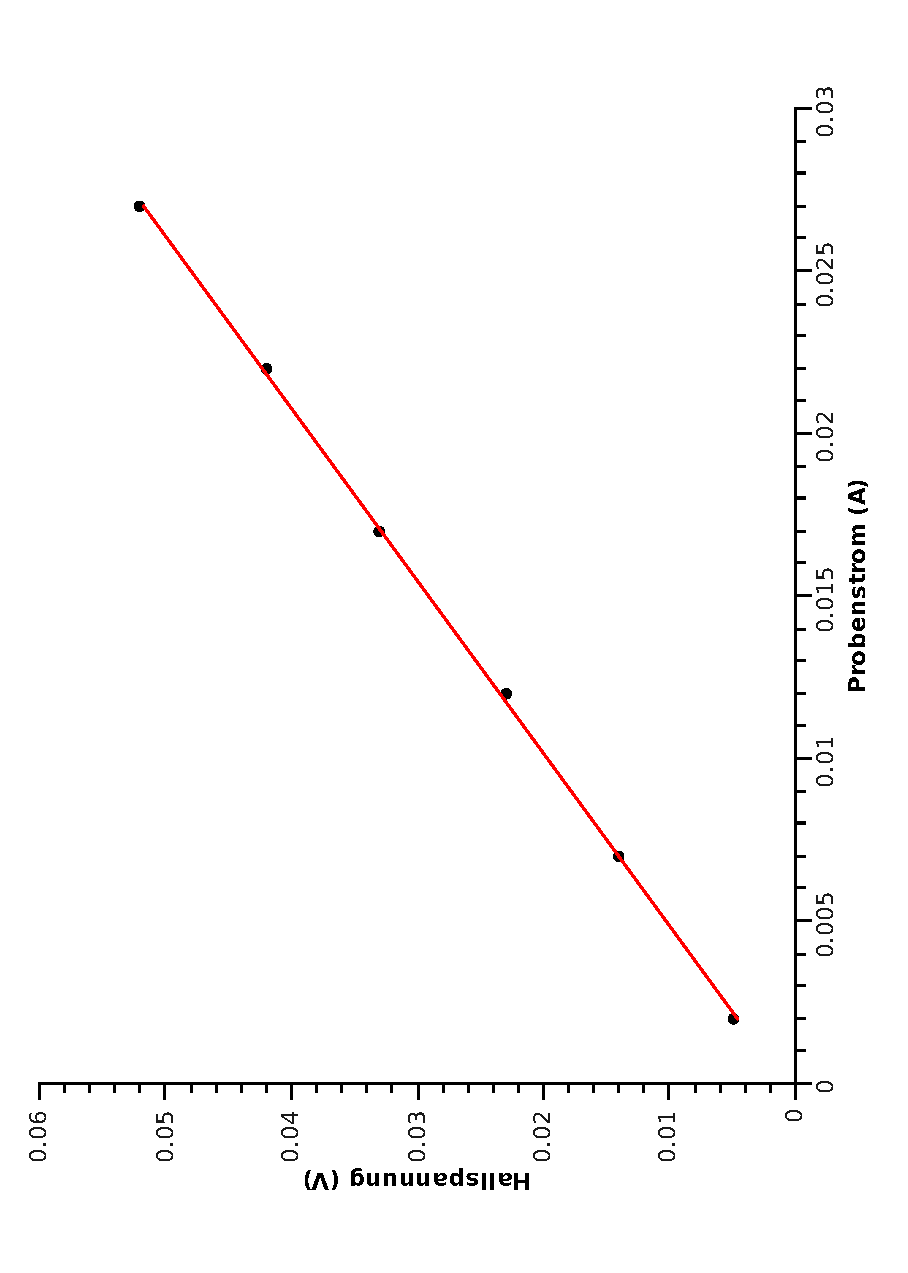
\includegraphics[width=0.4\textwidth, angle=-90]{probenstrom.eps}
\caption{Probenstromabhängige Hallspannung}
\end{center}
\end{figure}

\begin{figure}[H]
\begin{subfigure}{0.4\textwidth}
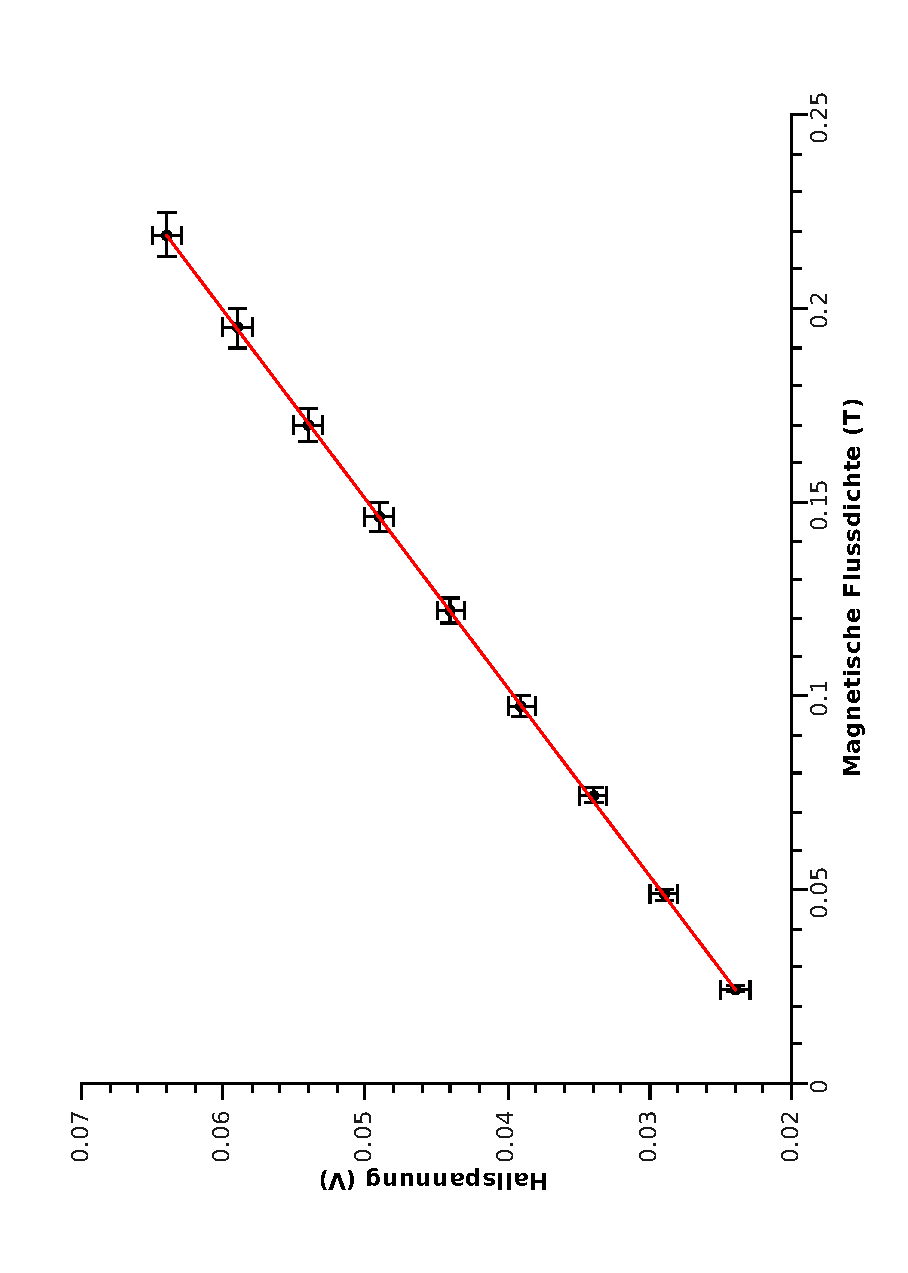
\includegraphics[width=0.9\linewidth, angle=-90]{npe.eps}
\caption{n-Ge}
\end{subfigure}
\begin{subfigure}{0.4\textwidth}
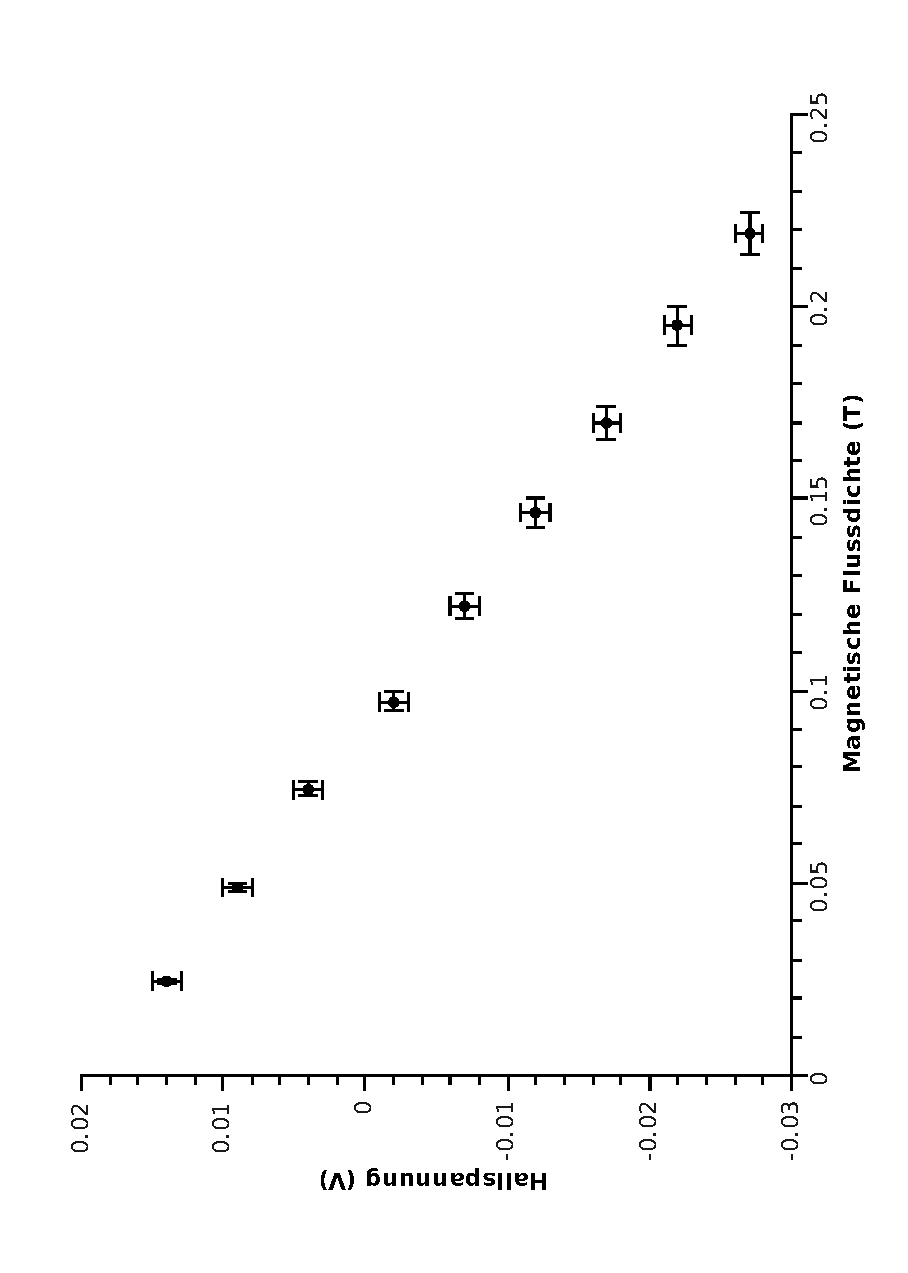
\includegraphics[width=0.9\linewidth, angle=-90]{npeumpol.eps}
\caption{n-Ge mit umgepoltem B-Feld}
\end{subfigure}
\\
\begin{subfigure}{0.4\textwidth}
\includegraphics[width=0.9\linewidth, angle=-90]{ppe.eps}
\caption{p-Ge}
\end{subfigure}
\begin{subfigure}{0.4\textwidth}
\includegraphics[width=0.9\linewidth, angle=-90]{ppeumpol.eps}
\caption{p-Ge mit umgepoltem B-Feld}
\end{subfigure}
\end{figure}


\begin{figure}[H]
\begin{center}
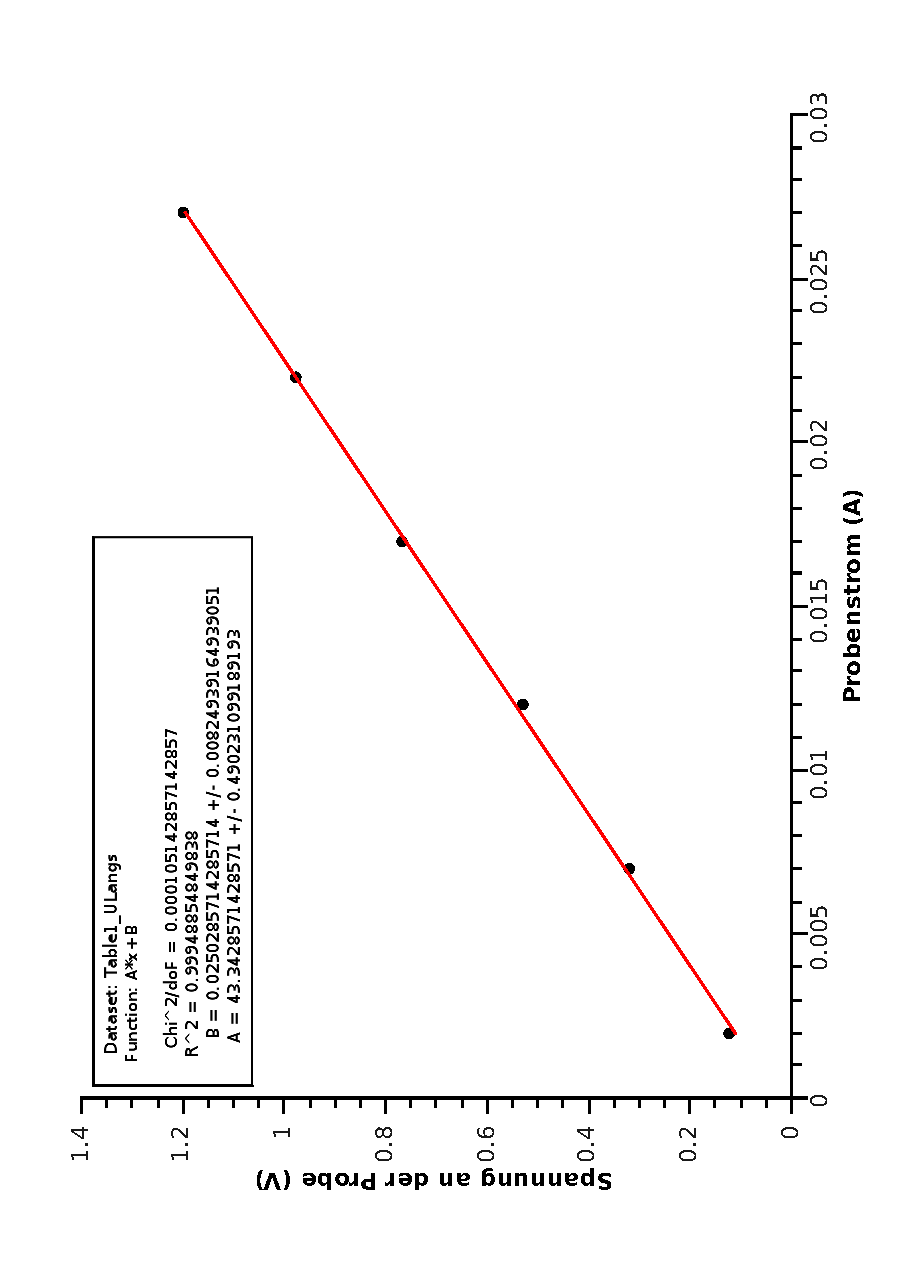
\includegraphics[width=0.4\textwidth, angle=-90]{widerstand.eps}
\caption{Probenspannung gegen Strom, die Steigung ist der Widerstand }
\end{center}
\end{figure}


\begin{figure}
\begin{subfigure}{0.4\textwidth}
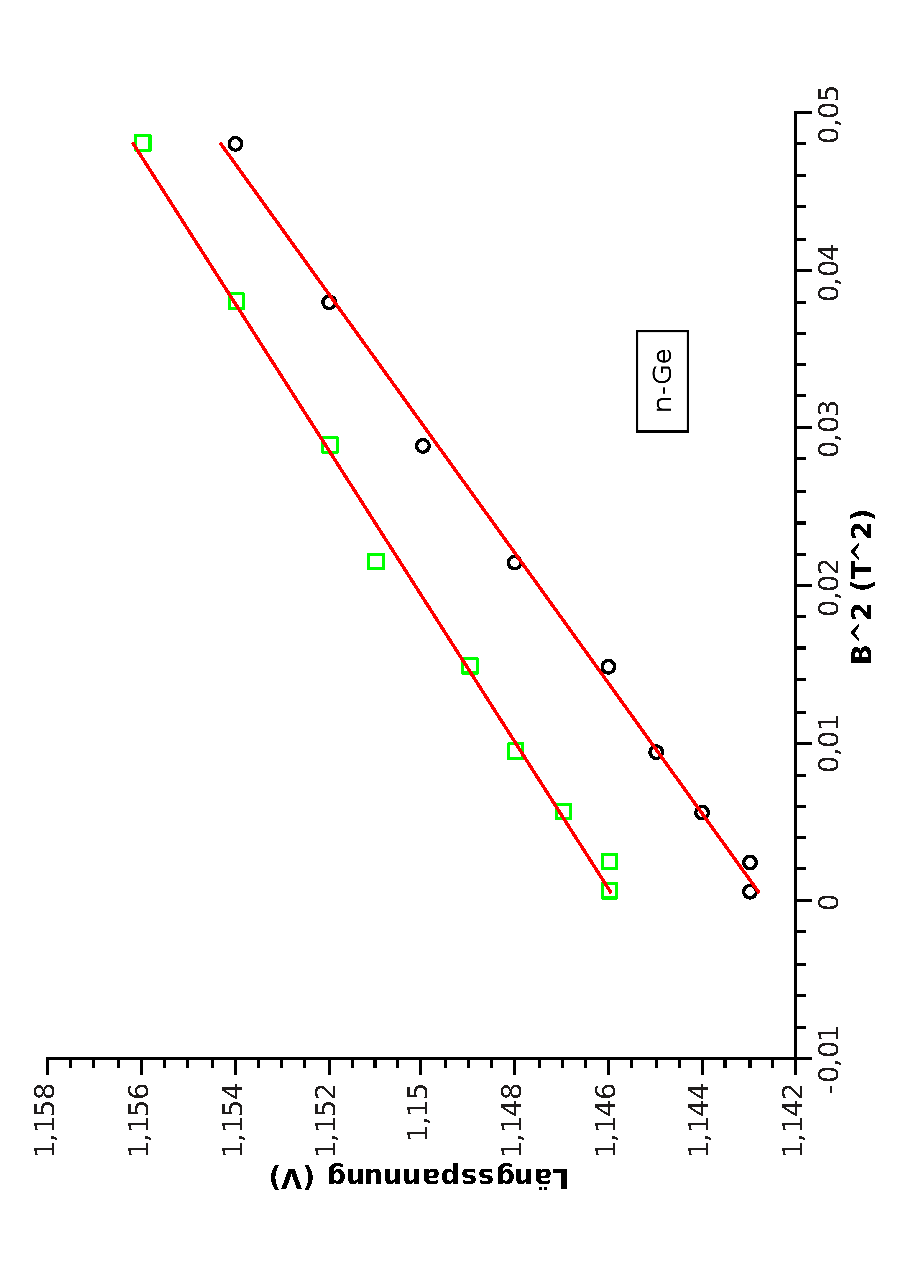
\includegraphics[width=0.9\linewidth, angle=-90]{magneton.eps}
\caption{Magnetowiderstand an n-Ge}
\end{subfigure}
\begin{subfigure}{0.4\textwidth}
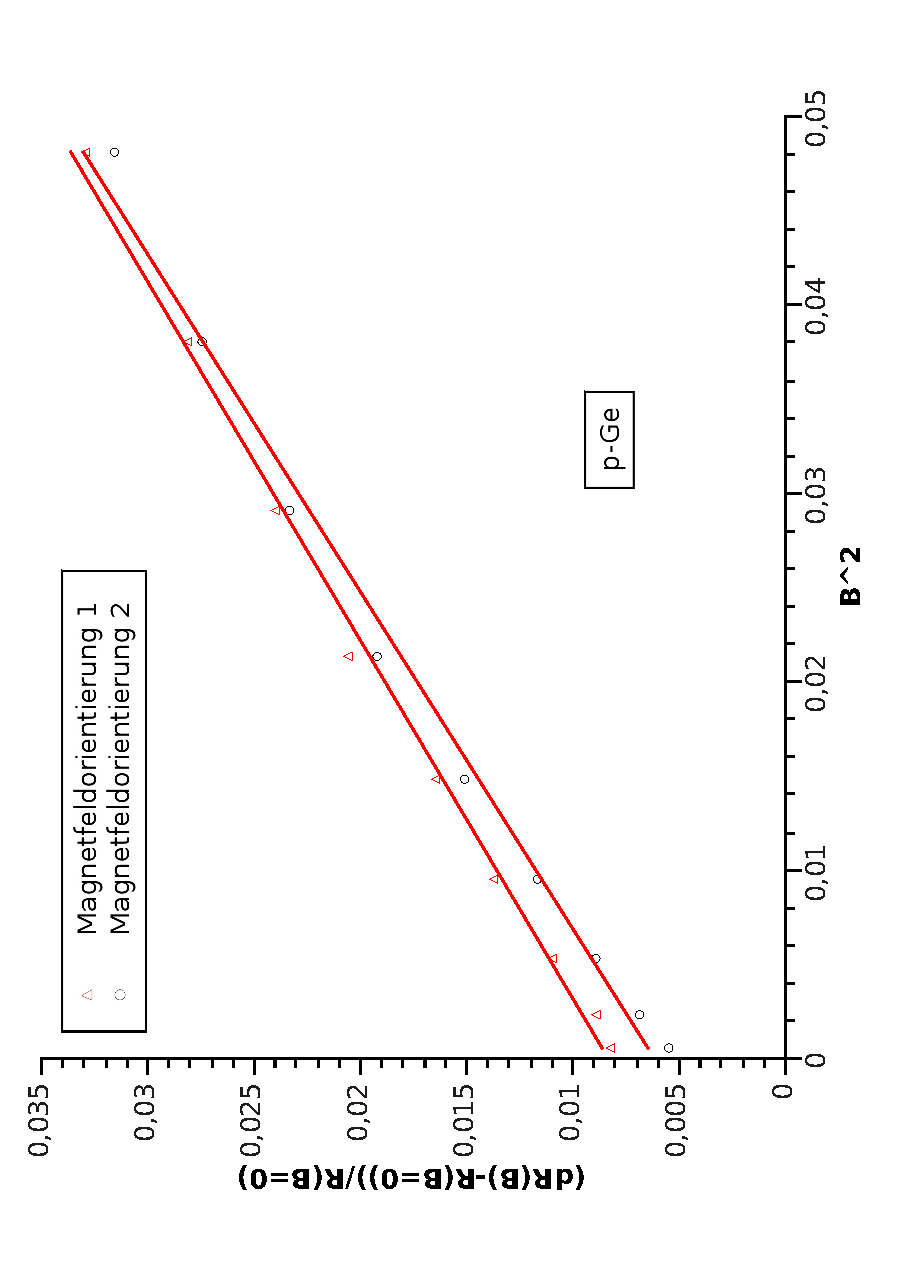
\includegraphics[width=0.9\linewidth, angle=-90]{magnetop.eps}
\caption{Magnetowiderstand an p-Ge}
\end{subfigure}
\caption{Längsspannung gegen $B^2$}
\end{figure}


\section{Diskussion}		

Durch Auftragung der Längsspannung gegen das Quadrat der Magnetischen Flussdichte, wie das erweiterte Modell vorhersagt, erkennt man sofort den Magnetowiderstand: Die Werte liegen auf einer Geraden.
																								
\end{document}